% !TEX root = ./geography.tex

\chapter{Global Sustainability \hspace{0.5em} Aquaculture}

\section{Syllabus}
	\textbf{Sustainability in the contemporary world}
	\begin{itemize}
		\item Sustainability and sustainable development, including pillars of sustainability - social, economic, environmental and cultural
		\item Principles of ecologically sustainable development - precautionary principle, intergenerational equity, conservation of biological diversity and ecological integrity
		\item Opportunities and challenges in planning for and achieving global sustainability \\ Including:
		\begin{itemize}
			\item the role of global forums, agreements and cooperation
			\item levels of action at a range of scales, from the United Nations Sustainable Development Goals to practices in local communities, including actions by governments, intergovernmental organisations (IGOs), non-government organisations (NGOs), corporations, community organisations and individuals
			\item Indigenous Peoples' practices and benefit sharing 
			\item political, economic, technological, social, cultural and environmental influences
		\end{itemize}
	\end{itemize}

	\textbf{Evaluating sustainability}
	\begin{itemize}
		\item The reasons for evaluating and monitoring global sustainability
		\item A range of criteria for evaluating the sustainability of economic activities
	\end{itemize}
	
	\textbf{Investigation of a global economic activity}

	Students study ONE global economic activity, for example:
	\begin{itemize}
		\item agriculture
		\item energy production
		\item fishing
		\item forestry
		\item manufacturing
		\item mining
		\item tourism.
	\end{itemize}

	For the global economic activity studied, students:
	\begin{itemize}
		\item evaluate the sustainability of the activity, using one or more criteria
		\item examine a range of strategies for sustainability
		\item critically analyse ONE strategy.
	\end{itemize}
	Students investigate:
	\begin{itemize}
		\item The nature and spatial patterns of the global economic activity
		\item Influences on the global economic activity \\ Including:
		\begin{itemize}
			\item biophysical
			\item economic
			\item technological
			\item political/organisational
		\end{itemize}
		\item Current trends and future directions
	\end{itemize}

\section{Relevant Statistics}
	\subsection{Nature}
		\begin{itemize}
			\item Total aquaculture production in 2022 was 130.9 million tonnes
			\item 2022 was the first time that global aquaculture surpassed capture production
			\item 59.1 million tonnes of production from inland water aquaculture
			\item Technological advancements in pond-based aquaculture have been adopted, increasing efficiency and reducing environmental impact. Eg. the in-pond raceway system ($\uparrow$production, $\downarrow$waste accumulation) is being increasingly adopted in China
			\item The 564 farmed species are taxonomically recognised 
		\end{itemize}
		
	\subsection{Spatial Patterns}
		\begin{itemize}
			\item Concentrated in Asia due to abundance of coastlines
			\item China's share in aquaculture reached 80.3\% in 2022
		\end{itemize}
		
		\begin{figure}[H]
			\centering
			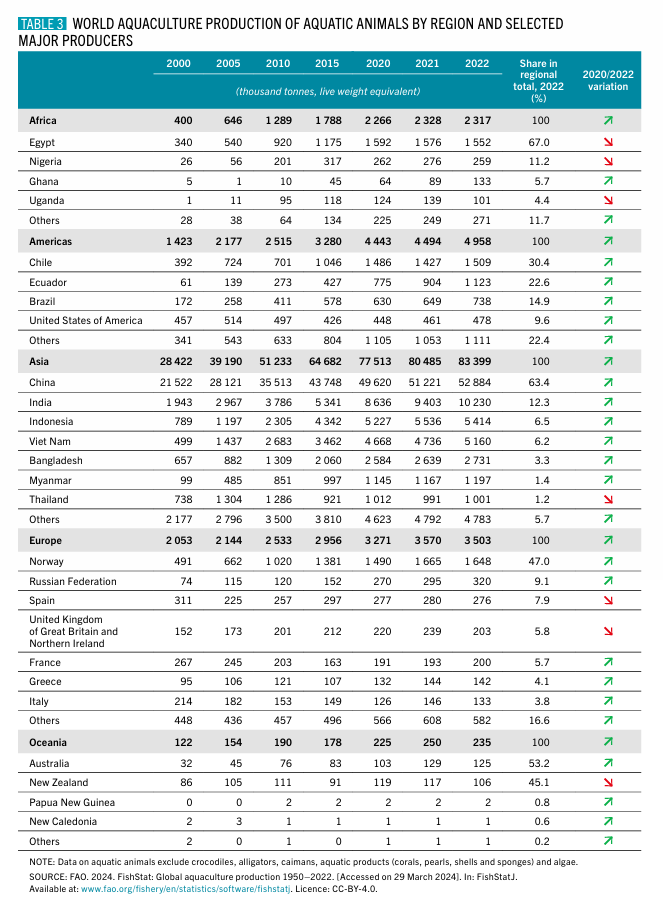
\includegraphics[width=15cm]{world aquaculture production of aquatic animals.png}
		\end{figure}

	\subsection{Environmental}

	\subsection{Economic}
	\begin{itemize}
		\item Global trade had value of USD 312.8 billion in 2022
	\end{itemize}

	\subsection{Social}
		\begin{itemize}
			\item In 2022, an estimated 61.8 million workers were employed in commercial fisheries and aquaculture
			\begin{itemize}
				\item Predominantly from Asia 85\%
			\end{itemize} 
			\item Aquaculture provided employment for around 22 million people
		\end{itemize}

	\subsection{Political}

	\subsection{SDGs}
		\textbf{SDG 2: Zero Hunger} - Aquaculture provides for 50\% of global seafood production. Sustainable aquaculture can reduce hunger and malnutrition, especially in developing countries due to their significant source of protein and micronutrients.

		\textbf{SDG 8: Decent Work and Economic Growth} - The aquaculture industry provides jobs for millions of people worldwide, from hatcheries to processing facilities.

		S\textbf{DG 12: Responsible Consumption and Production} - Aquaculture systems must be managed sustainably to avoid overuse of natural resources, reduce waste, and ensure efficient production. Promoting environmentally responsible practices like \textit{integrated multi-trophic aquaculture (IMTA)} minimizes negative ecological impacts while maximising yield.

\newpage

\section{Introduction to Aquaculture} \label{1/11/2024}
	"Farming of aquatic species in controlled or semi-controlled conditions"
		Eg. Salmon, barramundi, lobsters (can be semi-controlled), crabs, prawns, oysters, scallops, seaweed
		Non food: pearl scallops, coral (people keeping pets), crocodile skin
		Pets: goldfish

	In situ $\rightarrow$ In the environment

	Ex situ $\rightarrow$ Isolated to the environment

	Eg. Oyster farms in situ may be affected by external factors like a sewage spill

	\subsection{History}
		Although the Brewarrina fish traps are one of the oldest human constructions, they aren't real farms
		Roman oyster farm
		Chinese carp farm

	Aquaculture is practised across a wide variety of locations and species. Can be:
	\begin{itemize}
		\item Marine (mariculture), estuary or freshwater (in-land)
			\subitem Mariculture is currently underutilised, vast ocean space that isn't being used
		\item In-situ or ex-situ
		\item Fin-fish, crustacean, molluscs, or plants (usually algae)
			\subitem Carp (trash fish)
		\item For human consumption, fishmeal, or fish oil
		\item For local consumption or for export earning
			\subitem Norway and Chile grow the majority of the world's salmon, and is exports
			\subitem Changes the nature that the fish grows
	\end{itemize}

	\begin{align*}
		\text{\Large Aquaculture is \textbf{NOT} fishing}
	\end{align*}

	 In 2018, aquaculture produced 114.5 million tonnes in live weight, with a total farm-gate sale value of US\$263.6 billion
	Aquaculture accounted for 46\% of the total seafood production and 52\% of fish for human consumption
	China produces and consumes the largest amount of aquaculture, but also more broadly Asian countries

	There aren't that many inland waters, so inland fisheries do not have a significant amount of production \footnote{Carp and tilapia are not nice - David Latimer}

	Types of Economic Activity
	\begin{itemize}
		\item Primary - Farming
		\item Secondary - Manufacturing, producing
		\item Tertiary - Distribution of goods, using produced goods
		\item Quaternary - Researcher of salmon
		\item Quaternary - Researcher of salmon
	\end{itemize}

	\subsection{Distribution of Aquaculture}
		Aquaculture is mainly centred around Asia, with China representing around 60\% of global aquaculture
		Aquaculture is mainly centred around Asia, with China representing around 60\% of global aquaculture
		Fish is common in South-east Asia, especially with river fish eg. Vietnam
		Other countries just catch their fish

		African countries do not have the development or GDP to farm fish. Culturally also doesn't eat fish
		\footnote{"I don't like river fish, it's gross" - David Latimer}

		Developing countries are increasing their share of international fish trade
		Countries with large fishing catches often have larger aquaculture production
		
		Various places have cultural preferences and natural advantages for the production of particular species
		\begin{itemize}
			\item Predominantly carp \footnote{"River fish have a bland, muddy flavour" - David Latimer, D1 river fish hater}
			\item Seaweeds
			\item Tilapia
			\item Oysters
			\item Clams
			\item Catfish
			\item Prawns - Warm species
			\item Salmons, trout, smelts - Salmon is expensive
			\item Freshwater fishes
		\end{itemize}

		As China gets richer and richer, they will seek to eat more expensive fish, therefore increasing the demand

\section{Draft Nature and Spatial Patterns Text} \label{4/11/2024 - 6/11/2024}
	The text below is a reasonable, band 4-5 response to the stimulus prompt \textbf{“Examine the nature and spatial patterns of ONE global economic activity”}. Use the FAO report below to help you edit the text into a strong Band 6 response, complete with a clear thesis, detailed information and vocabulary, and well structured paragraphs.  Your finished text should be around 300-500 words in length. 

	{\large Draft Text}

	Aquaculture is global economic activity whereby people grow fish for food and trade. Aquaculture takes places around the globe, giving people both food and money. 

	Aquaculture is really old, having been practised for years and years. However, people grow lots of different species today. It's important to state that aquaculture and fishing are different activities.

	The economic activity of aquaculture can be carried out in both rich and poor countries. However, different countries tend to practise aquaculture differently and for different reasons. Aquaculture is mostly practised in rich countries. 

	Aquaculture is also practised in different environments. Moreover, these different types of aquaculture are not growing at the same speed. Some types of aquaculture are growing much more rapidly than others. 

	{\large Comments}
	\begin{itemize}
		\item Use stats
		\item In an "examine the nature and spatial distribution" question, evenly allocate writing to each part
		\item Specify location; Asia is very broad but aquaculture is focused around only 5
	\end{itemize}

\section{Influences on the global economic activity} \label{8/11/2024}
	"How do different things affect the activity of aquaculture"

	Nature, spatial patterns, future changes, sustainability

	\begin{table}[htbp]
		\centering
		\begin{tabular}{ll}
			Biophysical & How the biophysical environment and ecosystems influence aquaculture \\
			Economic & Demand and supply factors \\
			Technological & New developments that increase sustainability \\
			Political/Organisational & How is it controlled \\
		\end{tabular}
	\end{table}

	\subsection{Biophysical Factors}
		There are 622 species recognised by the FAO as being produced by aquaculture with each species requiring its own specific biophysical requirements

		Local water conditions can impart "\textbf{merroir}" to seafood $\rightarrow$ the flavour it has

		Local conditions flavour specialisation and give places competitive advantages
		\begin{itemize}
			\item Atlantic Salmon production is dominated by cold deep waters found in Norway and Chile
			\item Salmonids have become the largest single fish commodity by value
			\item Shrimp production benefits from brackish, warm tropical waters
		\end{itemize}

		Ex situ aquaculture attempts to separate aquaculture from the biophysical environment by controlling for temperature and chemistry. However, it is difficult to reproduce the conditions cheaply

		\begin{figure}[H]
			\centering
			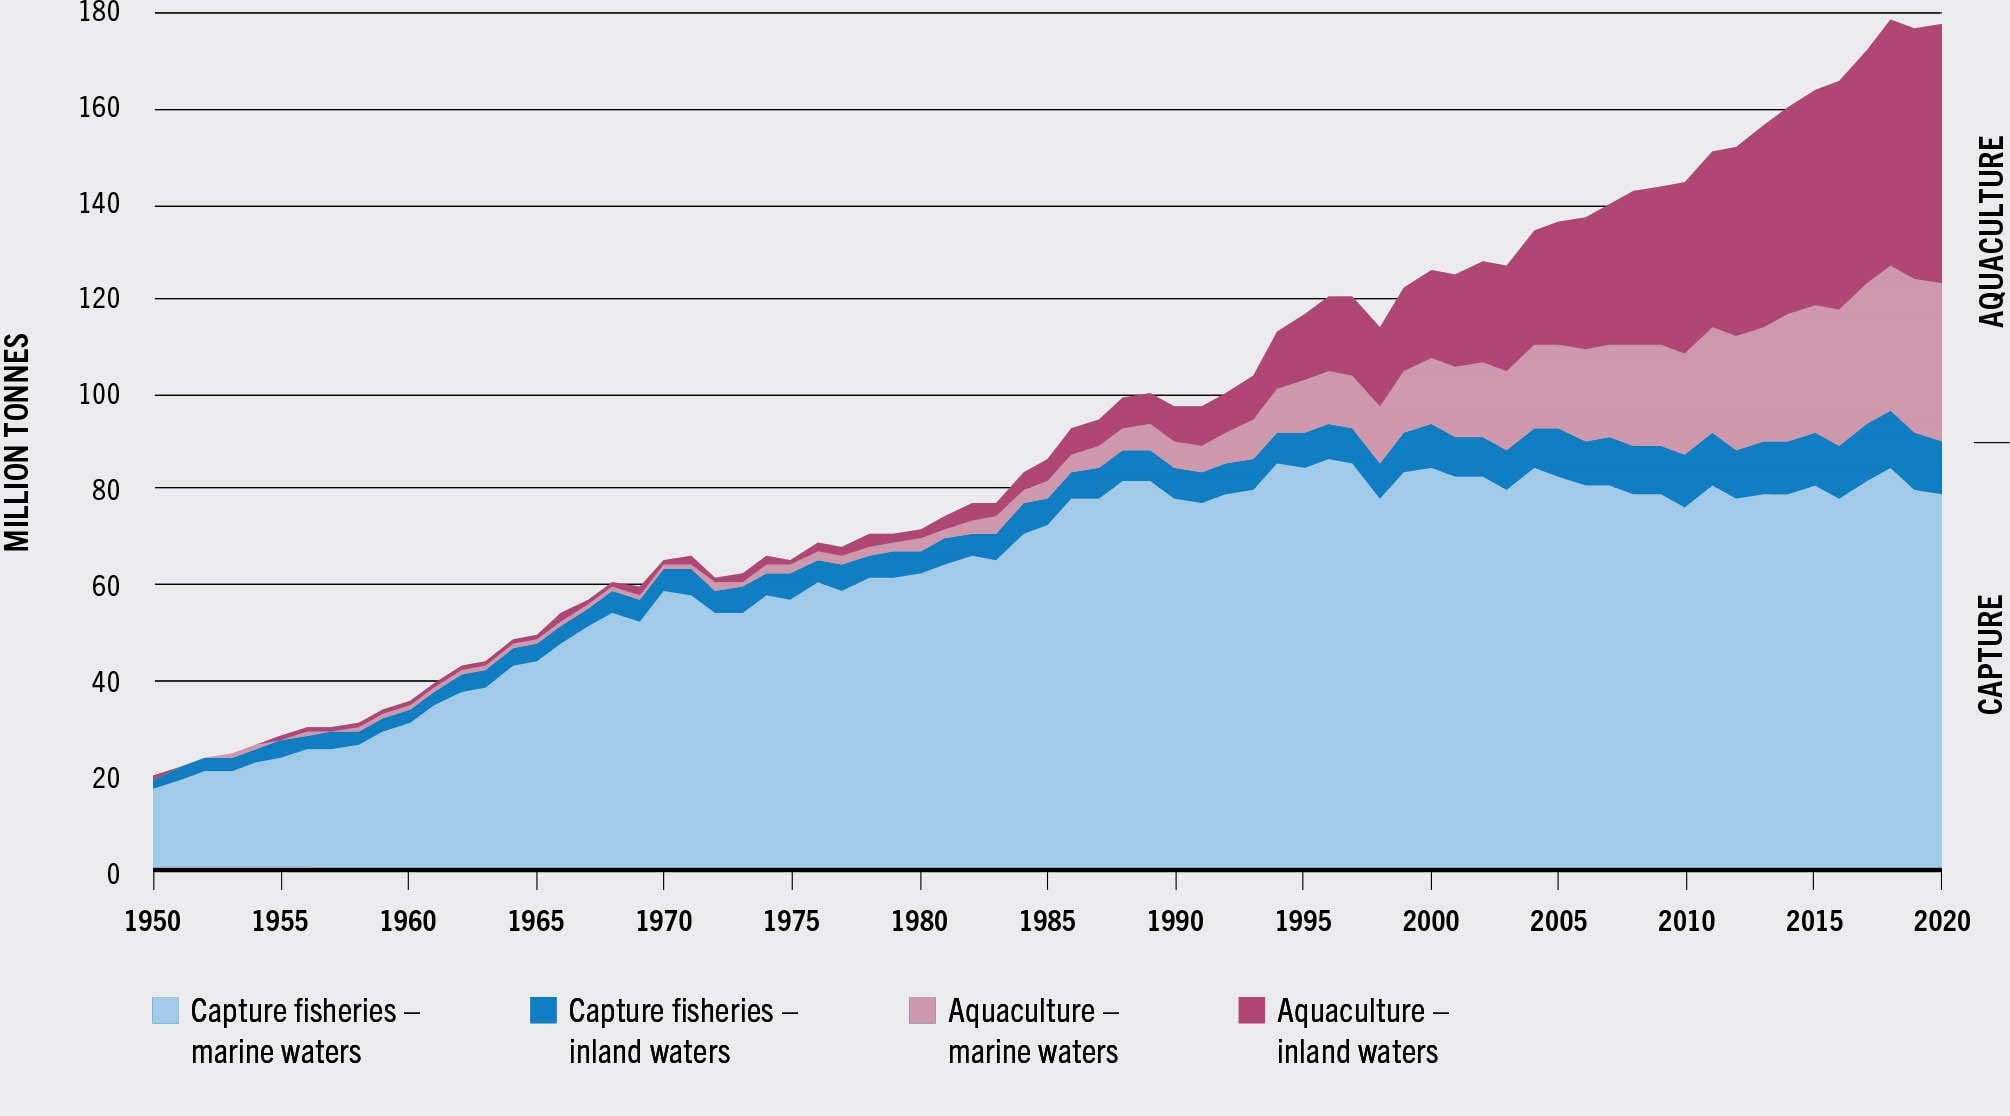
\includegraphics[width=15cm]{global fisheries and aquaculture graph.jpg}
		\end{figure}

		\subsubsection{Water Chemistry}
			The local bedrock and substrates will impact various chemical characteristics to the water, such as nitrates, phosphates, heavy metals
			Heavy metals are present due to mining operations that 

			Salinity is one of the most important characteristics of the water used in aquaculture
			\begin{itemize}
				\item Briny - High salinity
				\item Saline - Seawater, salt lakes
				\item Brackish - Estuaries, mangrove swamps
				\item Fresh - Ponds, lakes, river, streams
			\end{itemize}
		
			Eg. Oyster farmers will move their oysters up and down stream to control the way they grow

			Salmon farms need high flow of water to account for the waste produced by the high concentration of salmon
			Water plants can generally be grown anywhere

			\begin{figure}[H]
				\centering
				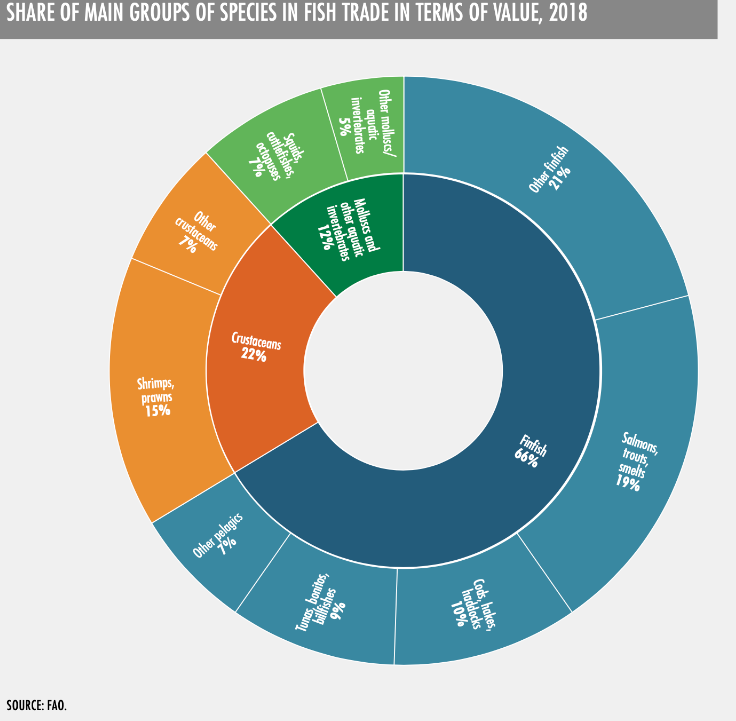
\includegraphics[width=15cm]{main groups of species in fish trade in terms of value.png}
			\end{figure}
			
		\subsubsection{Climate}
			Atlantic Salmon require deep water with temperatures below 10\textdegree C giving Norway and Chile an advantage

			Vannamei Shrimp require brackish, estuarine water that does not fall below 20 \textdegree C giving South-East Asian nations an advantage

		\subsubsection{Ecological}
			Aquaculture can have a highly detrimental interaction with local and global ecologies. For example:
			\begin{itemize}
				\item Carbon emissions from feed catch trawling
				\item By-catch from trawling
				\item Land clearing of mangroves
			\end{itemize}

			Aquaculture ventures often have to work with nearby human settlements. Some communities use this to produce multi-trophic production systems

			Disease outbreaks are increasing in aquaculture due to \textbf{monoculture}

			Eg. An in situ production system:
			\begin{itemize}
				\item Food pellets aren't completely consumed, increasing the concentration of food in an area
				\item The introduction of non-native species that are highly competitive
					\subitem Bad weather can increase the likelihood of escapes
				\item Predators like birds can attack birds, increasing the overall level of fish stress
				\item Bulk antibiotics applied to fish farms can impact resistance in future
					\subitem This can extend to humans consuming the fish 
				\item Fat salmon are better to eat, however to become this way they are overfed and lazy. If salmon escape, they can breed lazy salmon in the natural environment \footnote{"How do you get a fat salmon" - Latimer} \footnote{"You want a fat, lazy salmon" - Latimer}
			\end{itemize}

			To mitigate the greater environmental impacts:
			\begin{itemize}
				\item Make the farm ex situ
				\item Lower the density of the farm (However this lowers profit)
				\item Environmental Laws $\rightarrow$ Developing nations are also able to use lax environmental laws to develop coastal land for aquaculture
			\end{itemize}

			\textbf{Positive Ecological Impacts}

			Oyster farming industries can filter estuaries and apply pressure to keep waterways clean - encourages community to reduce pollution

		\subsection{Economic Factors}
			\subsubsection{Commodity Prices}
				Variable exchange rates and market prices for export commodities will modify production, including access to feed meal.

				In recent years, other major producing countries have reported low market prices of staple species, reflecting market saturation at least seasonally and locally for these mass-produced species.
				
				Salmon and avocado sushi was invented by Norwegians to encourage Japanese to purchase it
				Before introduction, Japan was not a major salmon consumer but was wealthy and Norwegians had an excess

				The \textbf{commodification} of aquaculture produce also placed demand to exceed environmental capacity. Commodification drives the production of more goods

			\subsubsection{Differences in HIC and LIC aquaculture}
				In some LICs, low labour costs can be a competitive advantage for production. 

				However, capital can be difficult to source in LICs - Greater degree of risk, less willingness for investors

				HICs will use the high value of their markets to demand higher quality produce.

				China has been accused of devaluing its yuan to promote exports. If their exchange rate is lower, their exports are cheaper, people will buy more, better for the Chinese market. (Denied by China ofc)
			
			\subsubsection{Urbanisation}
				People are increasingly living in cities with higher incomes and better infrastructure to facilitate fish purchases

			\subsubsection{Labour Specialisation}
				In HICs, changes in life expectations have made it difficult to find adequate labour - It is difficult to get people to work in far away aquaculture farms. Is promoted in Australia by using Tongan migrants as labour.

				In LICs, small scale farms account for much greater rates of production

				The International Labour Organisation (ILO) has identified that aquaculture utilises child and slave labour, but notes there is limited availability of evidence.

				People from Myanmar run to Thailand to escape the government. However questionable law enforcement in Thailand promotes illegal labour.
				One solution to this is international agreements and tariffs, however this is unlikely because people want their shrimp cheap. It is then a responsibility of the consumer to check the source of produce

		\subsection{Technological Factors} \label{11/11/2024}
			Selective breeding and GMO (genetically modified organism) technologies are common in aquaculture.

			Used to:
			\begin{itemize}
				\item Improve market appeal
				\item Address disease
				\item Promote growth
			\end{itemize}

			Often used in the salmon industry because salmon is more expensive

			Development in technologies for production are also important:
			\begin{itemize}
				\item Four stroke engine replacements $\rightarrow$ are less polluting than two stroke engines that release exhaust into the water, increasing pollution
				\item Optical scanner $\rightarrow$ can be used to replace human labour, ie. capital
				\item Improved cage netting $\rightarrow$ stronger materials for netting, double walled netting, overhead enclosure. Reducing escapees
			\end{itemize}

			\subsubsection{Transport and Retail Technologies}
				Improvements in refrigerated transport have boosted trade and consumption of aquaculture products.

				Internet sales and marketing have increased people's access to farm gate sales and reduced the cost and control of market sales. People are now able to purchase directly from the supplier, cutting out the middle man in trade.

				Geospatial technologies allow for tracking and more efficient trade.

		\subsection{Organisational Factors}
			International governance:
			\begin{itemize}
				\item Food and Agriculture Organisation (FAO) UN organisation that provides advice
				\item World Trade Organisation (WTO) polices trade
				\item International Labour Organisation (ILO) monitor conditions of labour
			\end{itemize}

			National scale:
			\begin{itemize}
				\item NSW Department of Primary Industries (DPI) peak controlling organisation, gives permits, permission
				\item NSW Food Authority eg. tells oyster farmers what they can and can't sell
			\end{itemize}

			The size of the Chinese market. Supply due to demand factors allows major traders to influence what is produced

			\subsubsection{Ownership}
				A wide variety of farm owners are responsible for global aquaculture production.

				Increasingly, large companies are looking to undertake \textbf{vertical and horizontal integration}
				
				As well as producers, in Australia, supermarkets are also able to control prices 
				Large aquaculture companies are able to use \textbf{economies of scale} to gain control over large market shares

				\textbf{Vertical integration}: Company aims to own the entire production process, however all the liabilities are placed on the company

				\textbf{Horizontal integration}: Company purchases competing companies in the same industry, eg. Cermaq is a major salmon and trout producer owned by Mitsubishi. For some companies, aquaculture is not their main goal, rather food in general

			\subsubsection{Control}
				 Supermarket chains exert significant power over consumers \footnote{The power of companies has always been extreme and have power in politics through funding}

				 Most people buy their food from supermarkets

			\subsubsection{Labelling and Decision Making}
				Sea food labelling rules change consumer preference and may require government intervention

				Australian made labels don't provide that much information about the product. If it is produced in many countries, the label will not say every country it has been in.

				Manufactured products are considered to be from that country. Eg. Malaysian prawns are labelled as Malaysian if raw, but if sauce is put on them in Australia, then they are manufactured in Australia

		\subsection{Political Factors}
			\subsubsection{International Trade}
				Tariffs are a tax on an imported good. Governments impose tariffs so the local businesses can compete with cheaper imports

				Subsidies are similar, but work in reverse. The government pays local farmers so that they can continue production. Protects domestic employment \\
					\; Eg. Sugarcane farmers in Queensland are given money to maintain employment. Queensland is a swing state, so governments are always going to provide funding
				
				A quota is a limit of number of items imported into a country.

				Import and export barriers to free trade are used to protect local industries.

				However, trade wars have also affected aquaculture products and commodity prices - particularly soybeans. \\
					\; Countries are likely to apply tariffs on each other, elevating economic tensions

				Diplomatic relationships and the WTO are important in resolving disputes

				The WTO also regulates Trade Regulated Intellectual Property Rights (TRIPS) which affects trademarks, geographic indications, patents and industrial designs \\
				\; A particular barramundi species can be patented, allowing you to market the quality of the barramundi

			\subsubsection{Asia-Pacific Trade}
				Australia participates in a range of bilateral and multilateral agreements which facilitate greater trade with the Asia-Pacific region.
				Trade relationships are often overlapping

				However, trade can also place environments at risk from exotic species and pathogens. It can cause confusion whether it is imposed as a biosecurity risk or as a trade restriction.

			\subsubsection{Legislation}
				Growth of aquaculture has outpaced the development of legislation and legal frameworks to govern the industry

				Land clearing has been unchecked in some places

				Development of a valuable industry has been given precedence over environmental concerns.

				Research, monitoring and lobbying by NGOs like Greenpeace and WWF provides political pressure on nation-states.

			\subsubsection{International Geopolitics}
				UNCLOS (1982) - Defines the 200 nautical mile boundaries for Exclusive Economic Zones (EEZ)

				Ramsar - Defines a number of internationally significant wetlands.

				CITES - Prevents trade of endangered species. For example the trade of illegally fished caviar from the sturgeon fish which is now mostly farmed.

				COP negotiations - Pressure on nations to change agriculture practices and prevent land clearing

				Nine dash line defined by China is still hotly contested due to fishing resources. China is a large country with large food demand

				Niger river catchment is the only source of water for some countries. Climate change means water is very important in the catchment. Conflict and destabilisation means that water resources are very valuable. The pollution of water resources due to aquaculture or the use of water in general could contribute to the conflict.

\newpage
\section{Practice Question}
	\textbf{Explain three influences that will likely determine the future directions of aquaculture globally. (6 marks)}

	Aquaculture is a rapidly developing global industry that has many opportunities for future growth. There are a variety of economic, technological and political influences that will likely determine the industry's future.

	Economic influences control how much the aquaculture industry can expand, with demand playing a vital role in the production of aquaculture products. Demand factors directly influence the funding resources that businesses have to continue and expand. If there is a lack in consumer demand for aquaculture products, there will be a decrease in production, and hence a contraction in the industry overall. Currently, the consumption of aquaculture products is generally similar the world, except for the highly concentrated popularity in East and South-East Asian countries, especially China. In 2024, China consumed 57,474 tons of fish, over four times higher than the second largest consumer, Indonesia. With the recent economic prosperity of the Asian region, the aquaculture industry has the ability to grow significantly to match the needs of its demand.

	Technological influences including emerging developments can also drive the growth of the aquaculture industry across the world. Developments in aquaculture often allow for more time and resource efficient production processes that maximise the affordability and viability of aquaculture. New technologies including the automation of processes such as feeding systems or water quality monitoring reduce impacts of human error, and can be cheaper to operate than using labour. This facilitates a more efficient operation, attracting potential investors and entrepreneurs. Emerging developments can also improve the environmental sustainability of aquaculture. For example, the transition from two-stroke to four-stroke boat engines increases fuel efficiency and can significantly reduce exhaust emitted into the water. Although four-stroke engines are not compatible in all situations, future technologies may further reduce waste generated from the aquaculture process. Technology hence has the ability to further expand the efficiency and sustainability of the aquaculture industry.

	The changing nature of the aquaculture industry requires new political legislations to maintain a sustainable and fair economic environment. Like other production industries, aquaculture requires land and other resources that can have external impacts to the wider ecosystem and community. Hence, some government organisations and NGOs advise and enforce rules upon businesses and nation states to maintain the sustainable growth of aquaculture. Currently, there are limited regulations surrounding the operation of aquaculture despite it being estimated to have reduced mangrove forests in countries such as Indonesia and Thailand by over 30\%. As well as this, it also increases the competition between countries for ocean areas. The South China Sea is a highly valuable area for potential aquaculture however is contested by its surrounding countries, with China extending its control over the region. With the increasing demand for food resources, areas such as this will need to be regulated to maintain equitable outcomes while still being available as a global commons.

\section{Sustainability} \label{14/11/2024}
	33\% of species are overfished, 60\% are fished at maximum capacity

	\subsection{Challenges to Sustainability}
		\begin{itemize}
			\item Capitalism drives over consumption and exploitation, caused and leading to commodification of aquaculture products
			\item Corporate control lacks respect for local values, ie. businesses are only interested in profit maximisation
			\item Ecological impacts can be externalised very easily, ie. negative externalities $\rightarrow$ social and environmental cost
			\item Lack of information and hence less consumer awareness limiting responsible purchasing decisions
		\end{itemize}

	\subsection{Issues with Aquaculture}
	\begin{itemize}
		\item Food chain bias with low conversion rates
			\begin{itemize}
				\item People mostly consume apex predators, ie. the top of the food chain eg. salmon
				\item Conversion rate is the efficiency of input to output of resources needed to produce a food $\rightarrow$ barramundi has high conversion rate, cows have low conversion rate
			\end{itemize}
		\item Monocultures lead to high disease mortalities
	\end{itemize}

	\subsection{Benefits of Aquaculture}
		\begin{itemize}
			\item Seaweed farms filter pollutants from the water, as well as absorb $\ce{CO2}$ from the air and water
			\item Aquaculture supports secondary and tertiary industries such as transport. This diversifies the economy, making it more resilient
		\end{itemize}

	\subsection{Economic Sustainability}
		Aquaculture has high export returns for national economies, especially prevalent in South and South-East Asian countries

		Developing countries have growing fish industries, increasing more rapidly than developed nations. Although this allows developing countries to reach developed status faster, its heightened growth may also be attributed to the lack of regulations regarding labour and land clearing.

		Aquaculture can create economic diversity through tertiary services such as:
		\begin{itemize}
			\item Consultation
			\item Resource management
			\item Infrastructure
		\end{itemize}
		This economic diversity provides more resilience and stability.

\section{Indigenous People's Practices and Benefit Sharing} \label{20/11/2024}
	\begin{itemize}
		\item Philosophical approaches
		\begin{itemize}
			\item Scientific knowledge
			\item Holistic approaches
		\end{itemize}
		\item Australian land management knowledge
		\begin{itemize}
			\item TUMRA
		\end{itemize}
		\item Potential medicines - Tea tree
		\item Potential foods
		\begin{itemize}
			\item Kangaroo
			\item Quandong
			\item Wattle seed
			\item Pepper bush
		\end{itemize}
	\end{itemize}

\section{ASC Label} \label{28/11/2024}
	\begin{itemize}
		\item The Aquaculture Stewardship Council (ASC) is an NGO acting as international standard setting and labelling body for responsible aquaculture.
		\item "informed consumers can improve the management of aquaculture by selecting products that are linked to high environmental and social production standards"
		\item Prevents misleading from self-claimed labels
		\item Established in 2010 by IDH (a Dutch sustainable trade initiative) and WWF Netherlands
			\begin{itemize}
				\item Introduced in Australia in 2017 with two part time staff \footnote{yay we have a grand total of \textbf{2} \textit{part time} staff in Australia :)}
			\end{itemize}
		\item Although Australia is a major producer of aquaculture, it usually exports high value seafoods (lobsters, abalone, tunas, scallops, prawns) but also imports lower value products (bulk fish, prawns)
		\item Greenwashing (untruly marketing as environmentally friendly, sustainable, or ethical) can occur in the aquaculture industry and is a concern for the ASC
		\item Self-created labels can be created cheaply and easily, therefore the ASC aims to provide as much information about goods, especially for imported products
	\end{itemize}

\section{Holiday Homework}
	\subsection{The EPBC Act}
		\begin{enumerate}
<<<<<<< HEAD
			\item Explain how the EPBC Act protexts threatened species in Australia?
=======
			\item Explain how the EPBC Act protects threatened species in Australia?
>>>>>>> cf81edad4e0473ec9bca6c1bfa03dacb39d68074
				\begin{itemize}
					\item When planning projects that impact natural environment/heritage (eg. mining, land clearing, property development, farming intensification), approval from Aust. govt and/or state+local govt.
					\item Mitigation strategies need to be accounted for
					\item Refer project to the department if there is significant impact
				\end{itemize}
<<<<<<< HEAD
				\subitem The EPBC enables the government to manage development projects that would impact the environment, as well as manaing nationally and internationally imported plants, animals, habitats, and places.
=======
				\subitem The EPBC enables the government to manage development projects that would impact the environment, as well as managing nationally and internationally imported plants, animals, habitats, and places.
>>>>>>> cf81edad4e0473ec9bca6c1bfa03dacb39d68074
				
				The Act protects certain nationally significant animals, plants, habitats, or places (protected matters). A referral and assessment may be required if a project potentially impacts matters protected under the EPBC Act.

				The Act protects nationally threatened species and ecological communities by:
				\begin{itemize}
					\item identifying high risk species and ecological communities
					\item developing conservation advice
					\item maintaining a register of critical habitats
					\item recognising key threats
				\end{itemize}
			\item Explain how the EPBC Act would apply to the salmon industry in Macquarie Harbour.
			\subitem The EPBC Act regulates and monitors the processes of salmon farms in Macquarie Harbour to minimise environmental impact. When building the farms, a referral and assessment would need to be provided to the Australian and Tasmanian Governments, as well as the West Coast Council. The assessment of the farm would then be analysed, with appropriate amendments. Requirements could include:
			\begin{itemize}
				\item limiting the density of fish
				\item designing and implementing appropriate technologies that mitigate fish escape
				\item limiting the use of chemicals such as vaccines, as well as mitigating the amount of lost feed
			\end{itemize}
			These processes may reduce the profitability of salmon farming in the harbour, however would minimise harm to the local ecosystem.
			\item 
		\end{enumerate}

	\subsection{Our World in Dad - Urbanisation}
		\begin{enumerate}
			\item Describe how urban areas are defined.
				\subitem Although there is no internationally standardised definition of an urban area, country-based statistics are still useful in demonstrating population changes. Although varying, countries often categorised an urban area based on the number of inhabitants, as well as other metrics such as infrastructure development or designated cities.
			\item Describe the change in urban populations since 2000.
				\subitem Global urban populations have experienced a constant growth since 2000 of 0.13\% per year. In 2007, the distribution of rural and urban residents equalised.
		\end{enumerate}
	\subsection{Urbanisation and the Future of Cities - TedEd}
		\begin{enumerate}
			\item Outline the major challenges for urban residents?
				\subitem With the consistent increase of urbanisation, demand for resources will become an increasingly large issue. Food, sanitation resources, and education will need to be properly provided for. This increase in demand will also require environmentally sustainable processes for food production and infrastructure development to allow for large-scale production. 
		\end{enumerate}
	\subsection{World Cities Report 2024}
		\begin{enumerate}
			\item Explain how cities can best mitigate climate change today.
				\subitem Climate change mitigation strategies in cities should incorporate diverse urban groups, and are more likely to produce inclusive solutions. For example, input from people in high climate risk areas is more likely to produce effective plans. Community-led programs should therefore be supported by higher governance levels, benefitting from community knowledge and targeted approaches, while fostering general community engagement.
			\item Outline which cities and city residents are considered climate vulnerable.
				\subitem Coastal cities are at high risk to the effects of climate change due to sea-level rise and exposure to more severe weather systems. Low socioeconomic residents often reside in the most climate-prone areas of cities, further disadvantaging them. As well as this, marginalised groups are more often impacted by climate change due to existing issues.
		\end{enumerate}
<<<<<<< HEAD
	\subsection{Cities and Climate Change: Making the Links - Tedx}
=======
	\subsection{Cities and Climate Change: Making the Links - TedX}
>>>>>>> cf81edad4e0473ec9bca6c1bfa03dacb39d68074
		\begin{enumerate}
				\item Outline the best things cities can do do to mitigate climate change.
					\subitem Good data and monitoring to create effective, effective budgeting, community support
				\item Explain how cities are leading climate action.
					\subitem Implementing local laws to incentivise large building owners to reduce total energy use. Reducing consumption of energy has a vital role in reducing associated carbon emissions, and may facilitate the transition to less efficient sustainable methods while technology continues to develop. Investing in sustainable energy sources where appropriate can also decrease carbon emissions that drive climate change. For example, solar panels are especially useful in cities exposed to long periods of bright sun, such as Sydney. Using environment specific sustainable energy production methods can improve efficiency of such systems and reduce overall emissions. Developing new methods of energy production that decreases the amount of current waste.
		\end{enumerate}
<<<<<<< HEAD
	\subsection{How will the next generation of cities addres the challenges of climate change?}
=======
	\subsection{How will the next generation of cities address the challenges of climate change?}
>>>>>>> cf81edad4e0473ec9bca6c1bfa03dacb39d68074
		\begin{enumerate}
			\item Explain what this video suggests is the best way for cities to mitigate climate change.
				\subitem The video identifies transport as a major contributor to greenhouse gas emissions that affect climate change. Use of power from car manufactures resulted in cities designed for cars, such as large distances between designated residential and commercial land. The primary method of mitigating this is through the adaptation of urban areas to facilitate access to public transportation and active transit would decrease the use of private cars, as well as encourage city development to focus on accessibility without cars.
			\item Explain how climate mitigation also fosters high liveability in cities?
				\subitem As mentioned, reduction in fossil fuel powered transportation systems can help mitigate released carbon emissions. Building highly walkable cities increases their liveability and build environments where public infrastructure is capable of accommodating all inhabitants to minimise reliance on privately owned transport such as cars.
		\end{enumerate}
	\subsection{AT Kearney Global Cities Report}
		\begin{enumerate}
			\item Outline what is being measured by the global cities report
				\subitem The global cities report aims to measure and analyse the connectivity of globally influential urban areas. Data is used to generate a Global Cities Index (GCI) that assesses the current state of connectivity for 156 cities.
		\end{enumerate}